\documentclass[12pt]{article}
%DIF LATEXDIFF DIFFERENCE FILE
%DIF DEL /home/jpalmer/vindels/Manuscript/Phylo-Feb15/supplement.tex     Tue May 21 01:12:10 2019
%DIF ADD /home/jpalmer/vindels/Manuscript/Phylo-current/supplement.tex   Tue May 21 01:12:10 2019

\usepackage[margin=1in]{geometry}
%\usepackage{times}
\usepackage{mathptmx}
\usepackage{setspace}
\usepackage{lineno}
\usepackage{capt-of}
\usepackage{subcaption}
\usepackage{enumitem}
\usepackage[normalem]{ulem}
\usepackage{verbatim}

% section labels
\usepackage[small,compact,explicit]{titlesec}

%[numbers,sort&compress]
%removed to get full size citations as per their request
\usepackage{natbib}


\usepackage{graphicx}
\graphicspath{{images/}} 

\usepackage{url}
\urlstyle{same}

\renewcommand{\ULthickness}{0.75pt}

\titleformat{\section} {\vspace{6pt}\large\bfseries}{\thesection} {12pt} {#1\vspace{-6pt}}
\titleformat{\subsection} {\bf}{\thesubsection} {0pt} {#1\vspace{-12pt}}
\titleformat{\subsubsection}[runin]{\vspace{0pt}\normalfont\normalsize\bfseries}{\thesubsubsection} {6pt} {#1}

\usepackage{color,soul}
\sethlcolor{yellow}
\newcommand{\todo}[2]{\hl{\textbf{#1:} #2}}
\usepackage{booktabs}

\parindent 0pt
\parskip 12pt


\makeatletter
\newenvironment{figurehere}
{\def\@captype{figure}}
{}
\makeatletter

\setcitestyle{aysep={}}

\usepackage{xr}
\makeatletter
\newcommand*{\addFileDependency}[1]{% argument=file name and extension
  \typeout{(#1)}
  \@addtofilelist{#1}
  \IfFileExists{#1}{}{\typeout{No file #1.}}
}
\makeatother
 
\newcommand*{\myexternaldocument}[1]{%
    \externaldocument{#1}%
    \addFileDependency{#1.tex}%
    \addFileDependency{#1.aux}%
}
\myexternaldocument{main}


\onehalfspacing
\pagewiselinenumbers
%DIF PREAMBLE EXTENSION ADDED BY LATEXDIFF
%DIF UNDERLINE PREAMBLE %DIF PREAMBLE
\RequirePackage[normalem]{ulem} %DIF PREAMBLE
\RequirePackage{color}\definecolor{RED}{rgb}{1,0,0}\definecolor{BLUE}{rgb}{0,0,1} %DIF PREAMBLE
\providecommand{\DIFadd}[1]{{\protect\color{blue}\uwave{#1}}} %DIF PREAMBLE
\providecommand{\DIFdel}[1]{{\protect\color{red}\sout{#1}}}                      %DIF PREAMBLE
%DIF SAFE PREAMBLE %DIF PREAMBLE
\providecommand{\DIFaddbegin}{} %DIF PREAMBLE
\providecommand{\DIFaddend}{} %DIF PREAMBLE
\providecommand{\DIFdelbegin}{} %DIF PREAMBLE
\providecommand{\DIFdelend}{} %DIF PREAMBLE
\providecommand{\DIFmodbegin}{} %DIF PREAMBLE
\providecommand{\DIFmodend}{} %DIF PREAMBLE
%DIF FLOATSAFE PREAMBLE %DIF PREAMBLE
\providecommand{\DIFaddFL}[1]{\DIFadd{#1}} %DIF PREAMBLE
\providecommand{\DIFdelFL}[1]{\DIFdel{#1}} %DIF PREAMBLE
\providecommand{\DIFaddbeginFL}{} %DIF PREAMBLE
\providecommand{\DIFaddendFL}{} %DIF PREAMBLE
\providecommand{\DIFdelbeginFL}{} %DIF PREAMBLE
\providecommand{\DIFdelendFL}{} %DIF PREAMBLE
\newcommand{\DIFscaledelfig}{0.5}
%DIF HIGHLIGHTGRAPHICS PREAMBLE %DIF PREAMBLE
\RequirePackage{settobox} %DIF PREAMBLE
\RequirePackage{letltxmacro} %DIF PREAMBLE
\newsavebox{\DIFdelgraphicsbox} %DIF PREAMBLE
\newlength{\DIFdelgraphicswidth} %DIF PREAMBLE
\newlength{\DIFdelgraphicsheight} %DIF PREAMBLE
% store original definition of \includegraphics %DIF PREAMBLE
\LetLtxMacro{\DIFOincludegraphics}{\includegraphics} %DIF PREAMBLE
\newcommand{\DIFaddincludegraphics}[2][]{{\color{blue}\fbox{\DIFOincludegraphics[#1]{#2}}}} %DIF PREAMBLE
\newcommand{\DIFdelincludegraphics}[2][]{% %DIF PREAMBLE
\sbox{\DIFdelgraphicsbox}{\DIFOincludegraphics[#1]{#2}}% %DIF PREAMBLE
\settoboxwidth{\DIFdelgraphicswidth}{\DIFdelgraphicsbox} %DIF PREAMBLE
\settoboxtotalheight{\DIFdelgraphicsheight}{\DIFdelgraphicsbox} %DIF PREAMBLE
\scalebox{\DIFscaledelfig}{% %DIF PREAMBLE
\parbox[b]{\DIFdelgraphicswidth}{\usebox{\DIFdelgraphicsbox}\\[-\baselineskip] \rule{\DIFdelgraphicswidth}{0em}}\llap{\resizebox{\DIFdelgraphicswidth}{\DIFdelgraphicsheight}{% %DIF PREAMBLE
\setlength{\unitlength}{\DIFdelgraphicswidth}% %DIF PREAMBLE
\begin{picture}(1,1)% %DIF PREAMBLE
\thicklines\linethickness{2pt} %DIF PREAMBLE
{\color[rgb]{1,0,0}\put(0,0){\framebox(1,1){}}}% %DIF PREAMBLE
{\color[rgb]{1,0,0}\put(0,0){\line( 1,1){1}}}% %DIF PREAMBLE
{\color[rgb]{1,0,0}\put(0,1){\line(1,-1){1}}}% %DIF PREAMBLE
\end{picture}% %DIF PREAMBLE
}\hspace*{3pt}}} %DIF PREAMBLE
} %DIF PREAMBLE
\LetLtxMacro{\DIFOaddbegin}{\DIFaddbegin} %DIF PREAMBLE
\LetLtxMacro{\DIFOaddend}{\DIFaddend} %DIF PREAMBLE
\LetLtxMacro{\DIFOdelbegin}{\DIFdelbegin} %DIF PREAMBLE
\LetLtxMacro{\DIFOdelend}{\DIFdelend} %DIF PREAMBLE
\DeclareRobustCommand{\DIFaddbegin}{\DIFOaddbegin \let\includegraphics\DIFaddincludegraphics} %DIF PREAMBLE
\DeclareRobustCommand{\DIFaddend}{\DIFOaddend \let\includegraphics\DIFOincludegraphics} %DIF PREAMBLE
\DeclareRobustCommand{\DIFdelbegin}{\DIFOdelbegin \let\includegraphics\DIFdelincludegraphics} %DIF PREAMBLE
\DeclareRobustCommand{\DIFdelend}{\DIFOaddend \let\includegraphics\DIFOincludegraphics} %DIF PREAMBLE
\LetLtxMacro{\DIFOaddbeginFL}{\DIFaddbeginFL} %DIF PREAMBLE
\LetLtxMacro{\DIFOaddendFL}{\DIFaddendFL} %DIF PREAMBLE
\LetLtxMacro{\DIFOdelbeginFL}{\DIFdelbeginFL} %DIF PREAMBLE
\LetLtxMacro{\DIFOdelendFL}{\DIFdelendFL} %DIF PREAMBLE
\DeclareRobustCommand{\DIFaddbeginFL}{\DIFOaddbeginFL \let\includegraphics\DIFaddincludegraphics} %DIF PREAMBLE
\DeclareRobustCommand{\DIFaddendFL}{\DIFOaddendFL \let\includegraphics\DIFOincludegraphics} %DIF PREAMBLE
\DeclareRobustCommand{\DIFdelbeginFL}{\DIFOdelbeginFL \let\includegraphics\DIFdelincludegraphics} %DIF PREAMBLE
\DeclareRobustCommand{\DIFdelendFL}{\DIFOaddendFL \let\includegraphics\DIFOincludegraphics} %DIF PREAMBLE
%DIF LISTINGS PREAMBLE %DIF PREAMBLE
\RequirePackage{listings} %DIF PREAMBLE
\RequirePackage{color} %DIF PREAMBLE
\lstdefinelanguage{DIFcode}{ %DIF PREAMBLE
%DIF DIFCODE_UNDERLINE %DIF PREAMBLE
  moredelim=[il][\color{red}\sout]{\%DIF\ <\ }, %DIF PREAMBLE
  moredelim=[il][\color{blue}\uwave]{\%DIF\ >\ } %DIF PREAMBLE
} %DIF PREAMBLE
\lstdefinestyle{DIFverbatimstyle}{ %DIF PREAMBLE
	language=DIFcode, %DIF PREAMBLE
	basicstyle=\ttfamily, %DIF PREAMBLE
	columns=fullflexible, %DIF PREAMBLE
	keepspaces=true %DIF PREAMBLE
} %DIF PREAMBLE
\lstnewenvironment{DIFverbatim}{\lstset{style=DIFverbatimstyle}}{} %DIF PREAMBLE
\lstnewenvironment{DIFverbatim*}{\lstset{style=DIFverbatimstyle,showspaces=true}}{} %DIF PREAMBLE
%DIF END PREAMBLE EXTENSION ADDED BY LATEXDIFF

\begin{document}



\begin{flushleft}

\baselineskip 24pt

{\Large Phylogenetic measures of indel rate variation among the HIV-1 group M subtypes: Supplementary Material}  % tentative

\end{flushleft}


\section * {Supplementary Figures}
%\todo{Art}{can't merge this title onto the next page with the GLM table}

\setcounter{table}{0}
\renewcommand\thetable{S\arabic{table}} 


\setcounter{figure}{0}
\renewcommand\thefigure{S\arabic{figure}} 


\begin{figure}[htbp]
    \centering
    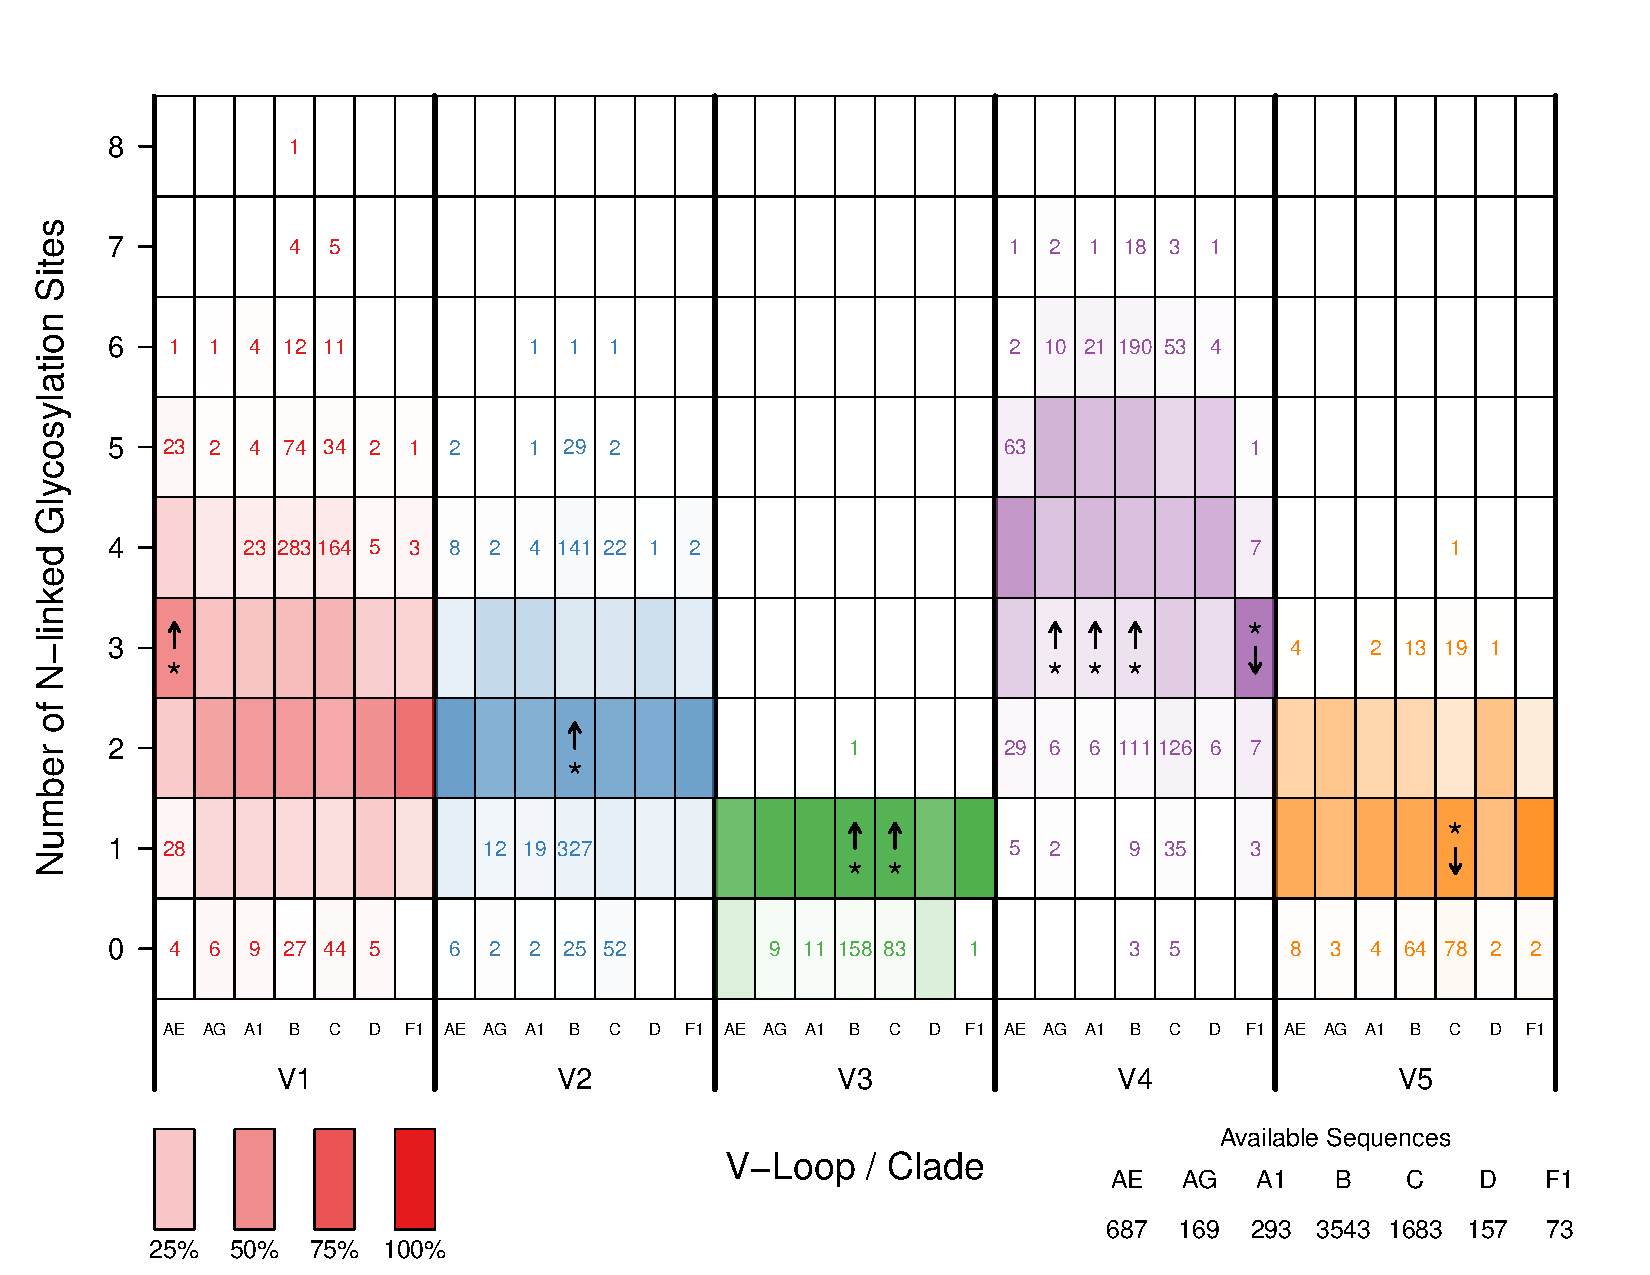
\includegraphics[width=.95\textwidth, trim={5mm, 0mm, 12mm, 15mm}, clip]{pngs-totals}
    \caption{The number of N-linked glycosylation sites in the variable loops of gp120.	
    Columns within each variable loop section describe the counts retrieved for one specific group M clade. 
    The color density of each box indicates the proportion of sequences containing the given count. 
    Examples of color densities and their corresponding proportions are provided by the four boxes to the bottom left of the figure.  
	Boxes containing a number highlight PNGS counts that are above zero, but contained less than 10\% of the distribution and therefore, did not generate a noticeable color.
    Asterisks (*) and arrows denote the presence and direction of significantly different PNGS counts among clades within a given variable loop (Poisson GLM).
    }
    \label{pngs-totals}
\end{figure}

\DIFaddbegin \begin{figure}[htbp]
    \centering
    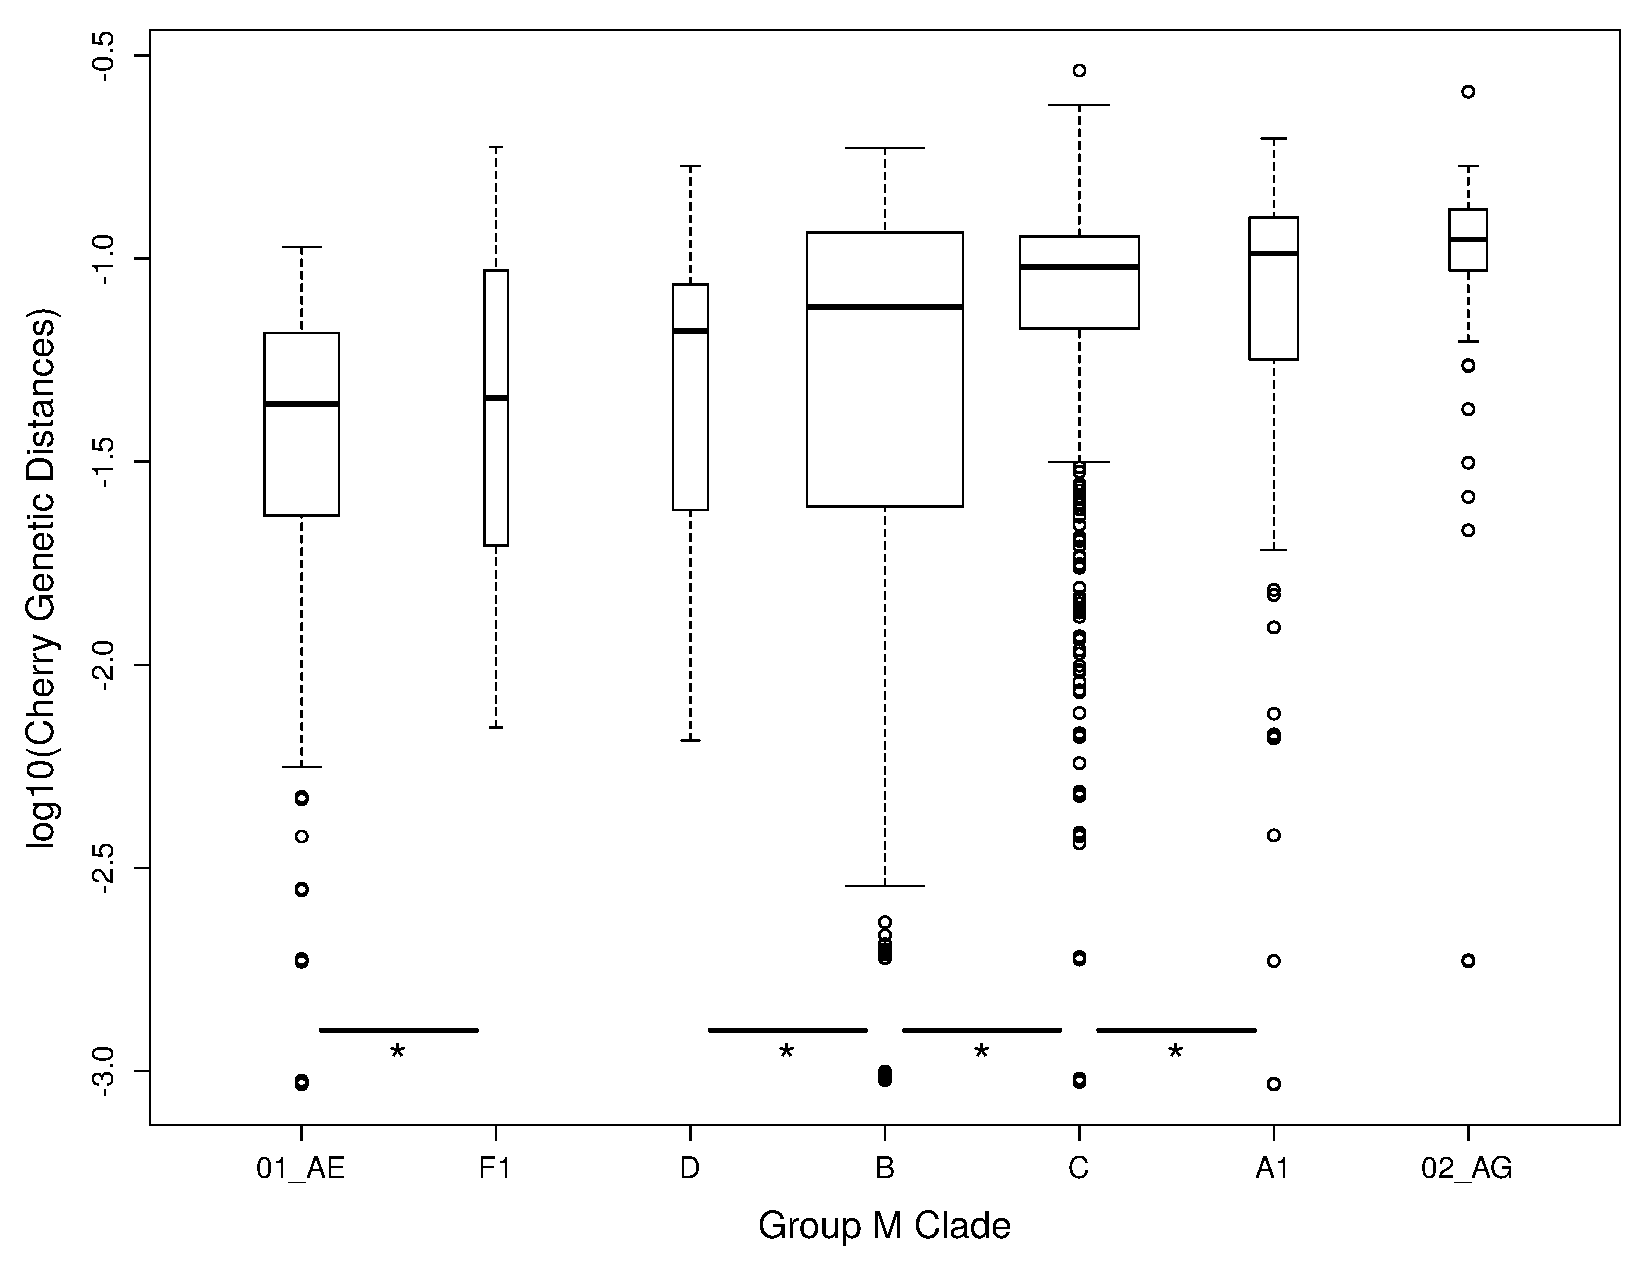
\includegraphics[width=.95\textwidth, trim={3mm, 0mm, 0mm, 0mm}, clip]{boxplot_logGD.pdf}
    \caption{ \DIFaddFL{Log$_{10}$-transformed genetic distances of sequences participating in cherries stratified by group M clade. 
    Box widths are representative of the number of cherry-derived sequences in the seven clades. 
    Sequences with zero genetic distance were excluded from this visualization. 
    For each clade in the order shown, counts of these filtered sequences were 16, 0, 6, 406, 24, 12, 24, and 2, respectively. 
    Although individual sequences had genetic distances of zero, no cherries in our data set had combined genetic distances of zero.}}
    \label{boxplot_GD}
\end{figure}

\DIFaddend \clearpage

\section * {Supplementary Tables}

\begin{table}[htbp]
\renewcommand{\arraystretch}{1.15}
  \centering
  \begin{tabular}{lrrcclrrc}
    \hline
   & Estimate & $P$ & Signif.   &&  & Estimate & $P$ & Signif. \\ 
    \cline{1-4} \cline{6-9}

    Time & 0.001 & $<10^{-15}$ & * & & Interactions \\ 
	Clade  &  &  &  &  & \hspace{1em}F1:V2 & -0.860 & 0.285 &  \\ 
  \hspace{1em}\DIFaddbeginFL \DIFaddFL{01\_}\DIFaddendFL AE &  (reference) &  &  && \hspace{1em}\DIFaddbeginFL \DIFaddFL{02\_}\DIFaddendFL AG:V3 & -2.073 & 0.063 &  \\ 
  \hspace{1em}\DIFaddbeginFL \DIFaddFL{02\_}\DIFaddendFL AG & 1.946 & 0.058 &  &  &\hspace{1em}A1:V3 & 0.127 & 0.799 &  \\ 
  \hspace{1em}A1 & -0.103 & 0.741 &  & &\hspace{1em}B:V3 & -0.381 & 0.255 &  \\ 
  \hspace{1em}B & -1.156 & $1.6\times 10^{-10}$ & * & &\hspace{1em}C:V3 & -0.109 & 0.752 & \\ 
  \hspace{1em}C & -0.372 & 0.065 & &&\hspace{1em}D:V3 & 1.363 & 0.017 &  \\ 
  \hspace{1em}D & -0.639 & 0.070 & &&\hspace{1em}F1:V3 & -13.565 & 0.926 & \\ 
  \hspace{1em}F1 & -0.158 & 0.780 && & \hspace{1em}\DIFaddbeginFL \DIFaddFL{02\_}\DIFaddendFL AG:V4 & -2.441 & 0.027 & \\ 
  Variable Region  & & & & &\hspace{1em}A1:V4 & -0.099 & 0.819 & \\ 
  \hspace{1em}V1 & (reference) & & & &\hspace{1em}B:V4 & -0.208 & 0.396 & \\
  \hspace{1em}V2 & -0.578 & 0.012 &  & &\hspace{1em}C:V4 & -0.215 & 0.428 & \\ 
  \hspace{1em}V3 & -4.448 & $<10^{-15}$ & * &  &\hspace{1em}D:V4 & 0.718 & 0.164 &\\ 
  \hspace{1em}V4 & -0.438 & 0.044 & & &\hspace{1em}F1:V4 & -0.577 & 0.439 &  \\ 
  \hspace{1em}V5 & -0.042 & 0.844 & & &\hspace{1em}\DIFaddbeginFL \DIFaddFL{02\_}\DIFaddendFL AG:V5 & -2.455 & 0.022 & \\ 
  Interactions & & & &&\hspace{1em}A1:V5 & -0.569 & 0.151 & \\ 
  \hspace{1em}\DIFaddbeginFL \DIFaddFL{02\_}\DIFaddendFL AG:V2 & -2.349 & 0.039 & & &\hspace{1em}B:V5 & 0.194 & 0.407 & \\ 
  \hspace{1em}A1:V2 & -0.457 & 0.313 &  &&\hspace{1em}C:V5 & 0.246 & 0.345 & \\ 
  \hspace{1em}B:V2 & -0.918 & $4.1\times 10^{-4}$& * & &\hspace{1em}D:V5 & -0.156 & 0.740 & \\ 
  \hspace{1em}C:V2 & -1.115 & $1.1\times 10^{-4}$ & * & &\hspace{1em}F1:V5 & -0.188 & 0.797 & \\ 
  \hspace{1em}D:V2 & -0.326 & 0.527 &  & &\\  

  \hline
  \end{tabular}

  \caption{
    Statistical comparisons generated by applying a generalized linear model to cherry indel analysis. 
    Comparisons made between clades and between variable regions were in relation to a reference group (\DIFaddbeginFL \DIFaddFL{01\_}\DIFaddendFL AE and V1, respectively). 
    Effects of clade and variable region interactions were compared to predicted mean values to detect significant differences. 
    Groups with * symbols denoted statistically significant differences based on a Bonferroni-corrected threshold suited for multiple comparisons ($\alpha$ = 0.05/n). 
    }
    \label{tab:glm}
\end{table}

\end{document}
